

\begin{subsection}{Introducción al problema}

En este problema nos situaremos en una provincia de Optilandia, donde las ciudades están conectadas por rutas bidireccionales. Algunas de estas rutas (en general las que representan caminos más cortos y/o directos entre las ciudades) han sido catalogadas con la categoría de premium, indicando que se encuentran en mejor estado y que reciben mejor mantenimiento que el resto. Para reducir los costos del mismo existen regulaciones que impiden que una empresa de transportes utilice más de $k$ rutas premium en un mismo envío. Transportex es una de estas empresas y ha solicitado nuestros servicios para encontrar el camino de mínimo costo entre 2 ciudades (una de origen, otra de destino) cumpliendo con estas restricciones, siempre que esto sea posible.

Escribiremos un algoritmo que reciba los datos de las ciudades, las rutas y el $k$ permitido y encuentre una solución si es que existe. Las ciudades pueden interpretarse como los nodos de un grafo, y las rutas que las conectan como las aristas del mismo, por lo que interpretaremos la entrada como un grafo; también se sabe que siempre hay una forma de llegar de una ciudad a otra (independientemente del uso de rutas premium), por lo que este grafo será conexo. Llamaremos $n$ a la cantidad de nodos del grafo y $m$ al número de sus aristas. 

A partir del mismo construiremos un digrafo en el que los nodos serán tuplas  $\langle c, p \rangle$, representando que se puede llegar a la ciudad $c$ utilizando a lo sumo $p$ rutas premium. As\'{i}, 2 nodos estar\'{a}n conectados sii se puede pasar de un estado a otro, formalmente,  si $c_1$ y $c_2$ est\'{a}n conectadas en el grafo de entrada, $\langle c_1, p \rangle$ y $\langle c_2, p \rangle$ estar\'{a}n conectadas si las une una ruta normal, y $\langle c_1, p \rangle$ y $\langle c_2, p + 1\rangle$ estar\'{a}n conectadas si las une una ruta premium. 

Se construye un digrafo y no un grafo ya que si $c_1$ y $c_2$ est\'{a}n conectadas por una ruta premium, tiene sentido poder avanzar desde $\langle c_1, p \rangle$ hacia $\langle c_2, p+1 \rangle$ pero no al rev\'{e}s. Este digrafo tiene $n(k+1)$ nodos ya que se genera un nodo $\langle c_1, p \rangle$ para cada $c_1 \in [0; n)$ y para cada $p \in [0; k]$; en cuanto a las aristas, se generarán a lo sumo $k$ por cada arista incidente a $c_1$ en el grafo de entrada (este número cambiará en función de qué rutas sean premium y cuales no). En total, la cantidad de aristas del digrafo es, a lo sumo, $mk$.

Finalmente, obtendremos el camino m\'{i}nimo entre $\langle origen, 0 \rangle$ y $\langle destino, p \rangle$, $0 \leq p \leq k$, es decir, el camino m\'{i}nimo desde el origen, sin haber usado rutas premium (en realidad no se han usado rutas de ning\'{u}n tipo) y el destino, habiendo usado a lo sumo $p$ rutas premium. Es preciso notar que $k$ es el máximo número de rutas premium a utilizar, y que los caminos que utilicen menos también deben ser considerados, tomando de entre ellos el de mínimo costo.

\end{subsection}


\begin{subsection}{Representaci\'{o}n}
Representamos al grafo de entrada como una lista de adyacencia: para cada nodo se guardan sus vecinos junto con sus respectivas distancias.  Para simplicidad guardaremos la información sobre las rutas premium de la siguiente manera: si $d$ es la distancia (en valor absoluto) entre 2 ciudades, $d$ se guardará con signo negativo si esas ciudades est\'{a}n unidas por una ruta premium, y positivo cuando las une una ruta normal. Notar que $G$ es un grafo a pesar de esta representaci\'{o}n, y que la ciudad numerada como $i$ en el archivo de entrada será numerada como $i-1$ en la lista de adyacencia.
El nuevo digrafo se representa también con lista de adyacencia, donde cada vecino tiene el nodo correspondiente y la distancia. Dado que la información sobre si una ruta es premium o no está contenida en la conexión entre los nodos, las distancias se guardan positivas. Por lo tanto, un vecino es una tupla $\langle nodo, distancia \rangle$, donde los nodos son las tuplas $\langle c, p \rangle$ descriptas anteriormente y las distancias son números naturales.

\end{subsection}

\begin{subsection}{El algoritmo}
El algoritmo que resuelve el problema consta de 2 partes: la primera es la construcción del digrafo descr\'{i}pto anteriormente y la segunda la ejecución del algoritmo de Dijkstra sobre el mismo para encontrar los caminos minimos. Mostramos a continuación el armado del digrafo:

\begin{algorithm}[H]
  \begin{algorithmic}[1]
    \Function{Problema1-armarDigrafo}{grafoDeEntrada: listaAdyacencia$\langle int, int \rangle$ grafoEntrada, n: int, origen: int, destino: int, k}
    \State  grafo $\gets$ listaAdyacencia$\langle nodo, distancia \rangle$ de n(k+1) nodos
    \For{$i \in [0; n])$}
        \For{$v \in$ grafoDeEntrada.\textproc{vecinosDe($i$)}}
            \For{$p \in [0;k]$}
                \If{$p \neq k \wedge$ $i$ y $\Pi_1(v)$ están conectadas por una ruta premium}
                \State grafo.\textproc{AgregarVecino}($\langle i, p \rangle, \langle \langle \Pi_1(v), p+1 \rangle, |\Pi_2(v)|\rangle$)
                \ElsIf{$i$ y $\Pi_1(v)$ \underline{\textit{no}} están conectadas por una ruta premium}
                \State grafo.\textproc{AgregarVecino}($\langle i, p \rangle, \langle \langle \Pi_1(v), p \rangle, |\Pi_2(v)|\rangle$)
                \EndIf
            \EndFor
        \EndFor
    \EndFor
    
    \State \textbf{return} \textproc{caminoMinimoDijsktra}($\langle origen,0\rangle, \langle destino, k \rangle, grafo, k$)
    \EndFunction    
  \end{algorithmic}
\end{algorithm}

\end{subsection}

Como solo nos interesa la distancia desde el origen hacia un nodo en particular, sería interesante poder cortar la ejecución de Dijsktra una vez que esa distancia ha sido hallada. Recordemos brevemente el algoritmo:

\begin{algorithm}[H]
\begin{algorithmic}[1]

\Function{AlgoDijsktra}{Grafo G, nodo origen, nodo destino}

    \State Inicializar $\Pi$ distancias y $Q$ cola de prioridades
    \While{$Q$ no está vacia}
        \State $u \gets$ min($Q$)
        \For {each $v$ vertice vecino de $u$}
            \State procesar $v$
        \EndFor
    \EndWhile
    \State \textbf{return} $\Pi(destino)$
\EndFunction

\end{algorithmic}
\end{algorithm}

Este algoritmo mantiene un invariante en el \textbf{while}: en el momento en el que un vértice $u$ es extraido de la cola, se sabe que se ha obtenido su distancia mínima al origen. Aprovechando esta característica, nuestra implementación de Dijsktra deja de iterar cuando la cola no tiene más elementos, o cuando algún nodo $\langle destino, p \rangle$ ha sido extraido de la misma. Dado que $0 \leq p \leq k$ por como se construye el grafo, cualquier nodo sirve, ya que la cantidad exacta de rutas premium usadas no es importante. El algoritmo final es el siguiente:

\begin{algorithm}
\begin{algorithmic}[H]

\Function{AlgoDijsktra}{Grafo G, nodo origen, nodo destino}

    \State Inicializar $\Pi$ distancias y $Q$ cola de prioridades
    \While{$Q$ no está vacia}
        \State $u \gets$ min($Q$)        
        \If{NumeroNodo($u$) $=$ NumeroNodo(destino)}
            \State \textbf{return} $\Pi(u)$
        \EndIf
        

        \algstore{dijsktra-final}
        
\end{algorithmic}
\end{algorithm}

\begin{algorithm}
\begin{algorithmic}

        \algrestore{dijsktra-final}

        
        
        \For {each $v$ vertice vecino de $u$}
            \State procesar $v$
        \EndFor
    \EndWhile
    \State \textbf{return} $\Pi(destino)$
\EndFunction

\end{algorithmic}
\end{algorithm}


\begin{subsection}{Complejidad}

Llamemos $D=(V',X')$ al digrafo generado por el algoritmo, $n'=n(k+1)$ a la cantidad de sus nodos y $m'=m(k+1)$ al número de sus aristas. La complejidad de la solución estará dada por las complejidades de sus 2 partes.:
\begin{itemize}

\item La generación del del digrafo cuenta con 3 ciclos anidados. El exterior itera sobre todos los nodos, luego el siguiente ciclo itera sobre cada uno de sus vecinos. Esto da un total de $2m$ iteraciones entre ambos \textbf{for}s. El ciclo interior (que itera sobre $p$) realiza $(k+1)$ iteraciones (cada una de tiempo constante) por cada vecino del nodo $i$, es decir que el digrafo se construye en $2m(k+1)$ iteraciones, lo cual es O($mk$).
\item El algoritmo de Dijsktra se implementa utilizando una cola de prioridad con actualización de prioridades en O(1) e inicialización y búsqueda de mínimo en O($t$) (donde $t$ es la cantidad de elementos de la cola, la cuál se corresponde con $n'$). Se harán $n'$ extracciones de mínimo y $m'$ actualizaciones de prioridades, obteniéndose una complejidad de O($(n')^2 + m'$), o lo que es lo mismo, O($(nk)^2 + mk$). 
\end{itemize}

Juntándose ambas las partes, el algoritmo correrá en O($(nk)^2 + mk$). Sabiendo que $m \leq n^2$, se puede afirmar que O($mk$) $\in$ O($n^2k$) $\in$ O($(nk)^2$).

\subsection{Correctitud}

Nuestra solución interpreta el mapa de entrada como un grafo $G=(V,X)$ y arma un digrafo $D=(X',V')$ para luego ejecutar el algoritmo de Dijskstra sobre él. Dado que éste algoritmo es correcto, bastará con demostrar que $D$ sirve efectivamente para resolver el problema. Llamemos $G_k$ al grafo (mapa) de entrada, restringido a los caminos que tienen hasta $k$ rutas premium, y $G - G_k$ al grafo (mapa) de entrada restringido a rutas de más de $k$ rutas premium. Demostrar que $D$ sirve para nuestro problema es equivalente a demostrar las siguientes 4 propiedades:


\begin{enumerate}
\item Todos los caminos de $G_k$ están en $D$
\item Todos caminos de $G - G_k$ no están en $D$
\item Para todo camino de hasta $k$ rutas premium, su costo en $G_k$ es el mismo que en $D$
\item Todos los caminos de $D$ están en $G_k$
\end{enumerate}

Si éstas propiedades son ciertas, buscar un camino mínimo en $G_k$ es equivalente a buscar un camino mínimo en $D$. 

Comencemos con algunas definiciones:
\begin{itemize}
\item Llamaremos $x_{ij} \in X$ a la arista que conecta los vértices $v_i$ y $v_j$ en $G$. 

\item Llamaremos $w(x)$ a la función de costo de las aristas de $G$ y $w'(x)$ a la función de costo de las aristas de $D$.

\item $(v_i, p) \in V'$, $\forall v_i \in V, \forall p \leq k$

\item Si $x_{ij}$ es una ruta premium, $\langle v_i, p \rangle$ estará conectada con $\langle v_j, p+1 \rangle$ en $D$ tal que $w(x_{ij}) = w'((\langle v_i, p\rangle, \langle v_j, p+1\rangle))$ (donde $p$ es la cantidad de rutas premium usadas hasta $v_i$ en el camino del que $v_i$ y $v_j$ son parte).

\item Si $x_{ij}$ es una ruta no premium, $\langle v_i, p \rangle$ estará conectada con $\langle v_j, p \rangle$ en $D$ tal que $w(x_{ij}) = w'((\langle v_i, p\rangle, \langle v_j, p\rangle))$ (donde $p$ es la cantidad de rutas premium usadas hasta $v_i$ en el camino del que $v_i$ y $v_j$ son parte).

\end{itemize}

Ahora sí, demostremos una a una las propiedades.

\subsubsection*{Los caminos de $G_k$ están en $D$.}

Sea $v_1, ..., v_n$ un camino $v_1$ hasta $v_n$ con $\lambda$ rutas premium, $v_i \in V$, $\lambda \leq k$. Notemos que este es un camino entre 2 nodos cualesquiera y que el nombre de los nodos es meramente orientativo, es decir, $n$ es la longitud del camino y $v_i$ es el $i$-ésimo nodo del mismo. Sea $P_1(n) = \exists (v_1, 0), ..., (v_n, \lambda )$ en $D$. Demostremos $(\forall n_0 \leq n)(P_1(n_0))$ por inducción en la longitud del camino.

\textbf{C.B.}: 
$P_1(1)$  es cierto pues $v_1$ es un camino de un único nodo, sin aristas, y se corresponde con el camino $(v_1, 0)$ en $D$.

\textbf{H.I.}: $P_1(t)$ es cierto $\forall t \leq n-1$

\textbf{T.I.}: 
\begin{itemize}

\item Si $x_{(n-1)n}$ es una ruta premium entonces el camino $v_1, ..., v_{n-1}$ utiliza $\lambda -1$ rutas premium. Por H.I. existe un camino de $(v_1, 0)$ a $(v_{n-1}, \lambda-1)$. Según las reglas de construcción del digrafo este nodo se conecta con $(v_{n}, (\lambda -1) + 1) = (v_{n}, \lambda)$. Entonces existe un camino de $(v_1, 0)$ a $(v_n, \lambda)$.

\item $x_{(n-1)n}$ es una ruta \textit{no} premium entonces el camino $v_1, ..., v_{n-1}$ utiliza $\lambda$ rutas premium. Por H.I. existe un camino de $(v_1, 0)$ a $(v_{n-1}, \lambda)$. Según las reglas de construcción del digrafo este nodo se conecta con $(v_{n}, \lambda)$. Entonces existe un camino de $(v_1, 0)$ a $(v_n, \lambda)$.

\end{itemize}

\subsection*{Todos caminos de $G - G_k$ no están en $D$}

Sea $v_1, ..., v_n$ un camino de $v_1$ hasta $v_n$ con $\lambda$ rutas premium, $v_i \in V$, $ k < \lambda$. Nuevamente, $n$ es la longitud del camino y $v_i$ su $i$-ésimo nodo. Sea $v_t$ un nodo de este camino, $t < n$, tal que $v_1, ..., v_t$ utiliza $k$ rutas premium y tal que $x_{t(t+1)}$ es una ruta premium. Este nodo existe porque el camino completo utiliza al menos $k+1$ rutas premium. Por $P_1(t)$ existe un camino $(v_1, 0)$ a $(v_t, k)$ en $D$. Según las reglas de construcción del digrafo, $(v_t, k)$ debe conectarse con $(v_{t+1}, k+1)$, pero este último nodo no pertenece a $D$ por definición, entonces el camino completo \textit{no} pertenece a $D$.

\subsection*{Para todo camino de hasta $k$ rutas premium, su costo en $G_k$ es el mismo que en $D$}

Sea $v_1, ..., v_n$ un camino de $v_1$ hasta $v_n$ con $\lambda$ rutas premium, $v_i \in V$, $ k < \lambda$, $n$ longitud del camino y $v_i$ su $i$-ésimo nodo. Sea $C_n = \sum_{i = 1}^{i \leq n-1} w(x_{i(i+1)})$ el costo total de este camino. Por $P_1(n)$ existe un camino $v_1' = (v_1, 0), ..., v_n' = (v_n, \lambda)$; sea $C_n' = \sum_{i = 1}^{i \leq n-1} w'((v_i', v_{i+1}'))$ el costo de este camino. Sea $P_2(n) = (C_n = C_n')$. Demostraremos $(\forall n_0 \leq n)(P_2(n_0))$ por inducción en $n$:

\textbf{C.B.}: 
$v_1$ es un camino de costo cero, pues no tiene aristas. $v_1'=(v_1, 0)$ es un camino de un único nodo que tampoco usa aristas y por tanto su costo también es cero. Luego $P_2(1)$ es verdadero. 

\textbf{H.I.}: $P_2(t)$ es cierto $\forall t \leq (n-1)$

\textbf{T.I.}: 
Por $P_1(n)$, $v_n' = (v_n, \lambda)$ es el último nodo del camino correspondiente en $D$. Por reglas de construcción del digrafo, el nodo anterior a éste es $v_{n-1}' = (v_{n-1}, p)$, con $p \in \{ \lambda, \lambda - 1 \}$, y se conecta con $(v_n, \lambda)$ mediante una arista de mismo costo que $x_{(n-1)n}$.

Por definición, $C_n = C_{n-1} + w(x_{(n-1)n})$ y $C_n' = C_{n-1}' + w'((v_{n-1}', v_n'))$. Por reglas de construción del digrafo, $w(x_{(n-1)n}) = w'((v_{n-1}', v_n'))$ y por H.I. $C_{n-1} = C_{n-1}'$, entonces $C_n = C_n'$.


\subsection*{Todos los caminos de $D$ están en $G_k$}

Sea $v_1', ..., v_n'$ un camino en $D$ tal que $v_n' = (v_n, \lambda)$, con $n$ la longitud del grafo y $v_i$ el $i$-ésimo nodo del camino. Sea $P_3(n) = \exists v_1, ..., v_n$ camino en $G$ de $\lambda$ rutas premium. Demostraremos $(\forall t \leq n)P_3(t)$ por inducción en la longitud del camino.  Como por definición $\lambda \leq k$, si $P_3(n)$ es verdadera entonces el camino estará en $G_k$.

\textbf{C.B.}: $v_1'$ es un camino de un único nodo que no usa ningún tipo de rutas, por lo tanto $\lambda = 0$ y $v_1' = (v_1, 0)$. Como $v_1 \in V$, $v_1$ es un camino de un único nodo en $G$ que usa 0 rutas premium. Por lo tanto $P_3(1)$ es verdadera. 

\textbf{H.I.}: $P_3(t)$ es cierto $\forall t \leq n-1$

\textbf{T.I.}: $v_n' = (v_n, \lambda)$ es el último nodo del camino. Por reglas de construcción del digrafo, el nodo anterior a este es o bien $(v_{n-1}, \lambda - 1)$ (y $x_{(n-1)n}$ es una ruta premium), o bien $(v_{n-1}, \lambda)$ (y $x_{(n-1)n}$ es una ruta no premium).

\begin{itemize}

\item Si el nodo anterior es $(v_{n-1}, \lambda - 1)$: Por H.I. existe $v_1, ..., v_{n-1}$ camino en $G$ con $\lambda - 1$ rutas premium. Como $x_{(n-1)n}$ es una ruta premium, el camino $v_1, ..., v_{n-1}, v_n$ utiliza $\lambda$ rutas premium.

\item Si el nodo anterior es $(v_{n-1}, \lambda)$: Por H.I. existe $v_1, ..., v_{n-1}$ camino en $G$ con $\lambda$ rutas premium. Como $x_{(n-1)n}$ es una ruta no premium, el camino $v_1, ..., v_{n-1}, v_n$ también utiliza $\lambda$ rutas premium.

\end{itemize}

Todas las propiedades son válidas, por lo tanto buscar el camino mínimo entre 2 nodos en $G_k$ es equivalente a buscarlo en $D$ y por tanto el digrafo no altera las soluciones. Luego el algoritmo es correcto. 

\subsection{Experimentaci\'{o}n}

Para la experimentaci\'{o}n realizamos un generador de instancias aleatorias para este problema, que genera grafos de $n$ nodos, $m$ aristas (de las cuales $p$ son premium) y busca un camino m\'{i}nimo de $origen$ a $destino$ usando $k$ rutas premium ($n, m, p, origen, destino, k$ son par\'{a}metros para el generador) . El algoritmo del generador puede ser simplificado en 3 pasos:
\begin{itemize}
    \item Generar un camino de $n$ nodos de manera aleatoria
    \item Generar aristas entre nodos aleatorios (siempre y cuando no estuvieran conectados previamente ni sean el mismo nodo) hasta completar a $m$ ($m$ se establece entre $n-1$ y $\frac{n(n-1)}{2}$).
    \item Seleccionar $p$ aristas aleatoriamente y catalogarlas como rutas premium.
\end{itemize}

Para generar el camino se selecciona un nodo aleatoriamente como inicial, y se lo marca como el nodo actual. Luego, sobre los nodos que no han sido seleccionados se selecciona un nuevo nodo aleatoriamente, se lo convierte en vecino del nodo actual y se lo marca como el nuevo nodo actual. Este proceso se repite hasta que no queden nodos que no hayan sido seleccionados. Para el segundo y tercer paso simplemente se seleccionan nodos aleatorios y se los une o marca su ruta como premium si las condiciones están dadas; en ambos casos se descartan aquellos nodos seleccionados y que no cumplan las condiciones para asegurar que el algoritmo termine. En cuanto a las condiciones, se unen nodos distintos que no hayan sido unidos previamente y se marca como premium el camino entre dos nodos sii estos están unidos y su ruta no es premium.
Para la selecci\'{o}n aleatoria se utiliza la funci\'{o}n \textproc{rand} de C++.

A continuación se harán experimentaciones para medir complejidades y para analizar casos buenos y malos para esta solución (en términos de complejidad).

\subsubsection{Mediciones de complejidad}

El objetivo de esta experimetaci\'{o}n es el de comprobar que las complejidades te\'{o}ricas se cumplan en la implementaci\'{o}n. Dado que la misma depende de las variables $n$, $k$ y $m$, se realizarán experimentaciones para medir cada una de ellas por separado, fijando las otras 2. Recordemos que la complejidad teórica analizada es de O($n^2k^2 + mk$), con $mk \in$ O($n^2k^2$).

\paragraph{Complejidad sobre $n$}

Para este primer experimento $k$ y $m'$ serán fijadas en 2000 y 20 respectivamente, mientras que $n$ aumentará de 100 hasta 500 dando saltos de a 10. Dicho de otro modo, se probarán instancias de tamaño $n = 100, 110, 120, ..., 500$, midiendo sus tiempos de ejecución. Para cada caso se harán 5 repeticiones y se tomará la mediana. Se espera que el crecimiento sea cuadrático, por lo que una vez obtenidos los resultados se calculará el coeficiente de pearson junto con las funciones $n$, $n^2$, $n^3$ y $n^4$ para medir la correlación de estas con los tiempos de corrida. Dado que todos son polinomios la correlación debería ser alta en todos los casos, pero $n^2$ debería tener la mayor correlación de acuerdo al análisis teórico. A continuación los resultados:

\hspace*{-1cm}{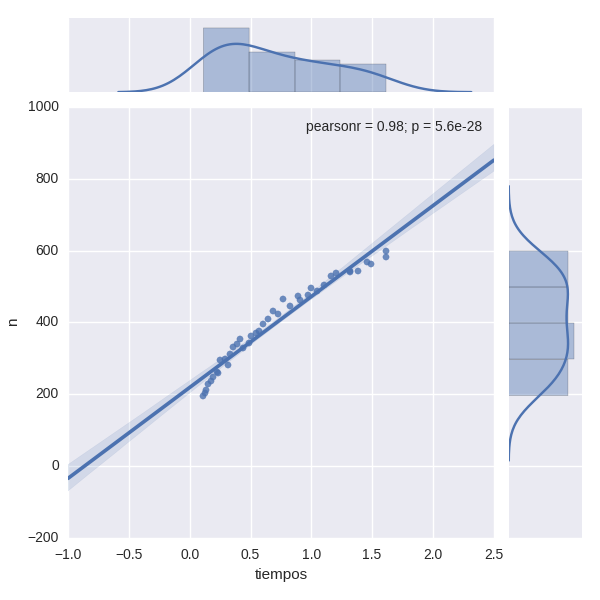
\includegraphics[width=8cm,height=8cm,keepaspectratio]{img/testn_n.png}}
\hspace*{-1cm}{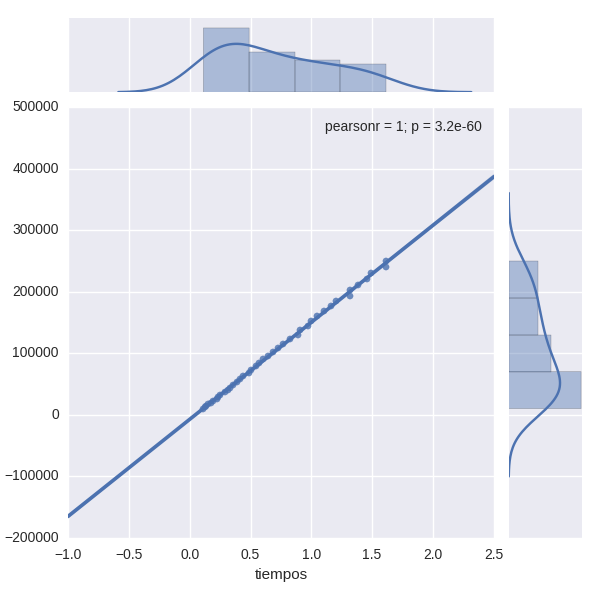
\includegraphics[width=8cm,height=8cm,keepaspectratio]{img/testn_n2.png}}

\hspace*{-1cm}{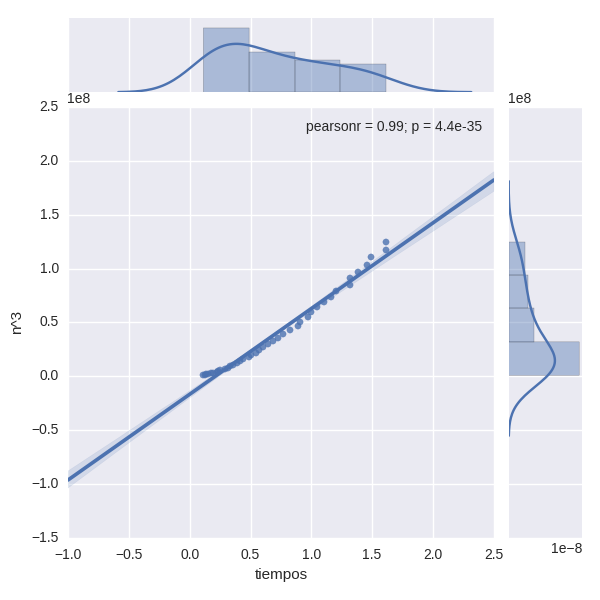
\includegraphics[width=8cm,height=8cm,keepaspectratio]{img/testn_n3.png}}
\hspace*{-1cm}{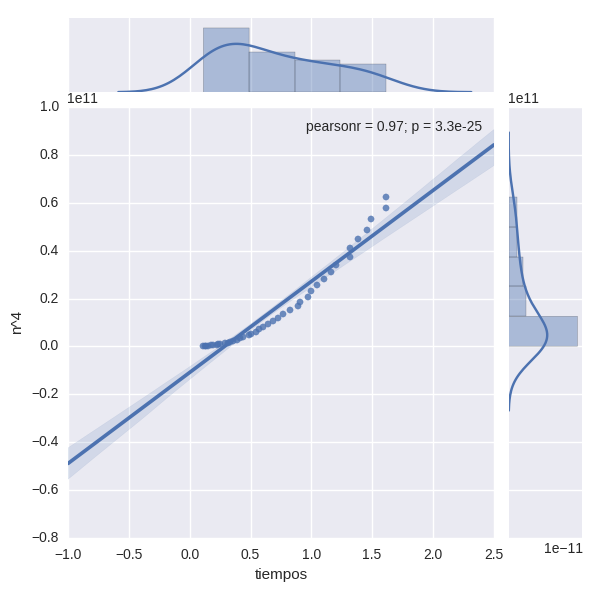
\includegraphics[width=8cm,height=8cm,keepaspectratio]{img/testn_n4.png}}

Tal como se esperaba, los coeficientes son altos en todos los casos, sin embargo la correlación entre los tiempos de corrida del algoritmo y la función $n^2$ es perfecta, por lo tanto el crecimiento de $n$ es cuadrático, tal como surgió del análisis teórico. Observar que la correlación con $n^3$ es casi perfecta (sin embargo con una probabilidad de error ligeramente mayor), lo cual sugiere que la constante que acompaña a la complejidad de la solución es grande en comparación con los tamaños de muestra y que con $n$ de mayor tamaño la diferencia será más notoria. 

\paragraph{Complejidad sobre $k$}

En este caso se fijarán $n$ y $m$ en 100 y 2000 mientras que $k$ aumentará desde 100 hasta 500 dando saltos de a 10. Nuevamente se miden tiempos de ejecución, se realizan 5 repeticiones para caso (tomando la mediana de las 5), y se mide la correlación con $n$, $n^2$, $n^3$ y $n^4$ mediante el coeficiente de pearson. También en este caso se espera que el crecimiento sea cuadrático. 

\hspace*{-1cm}{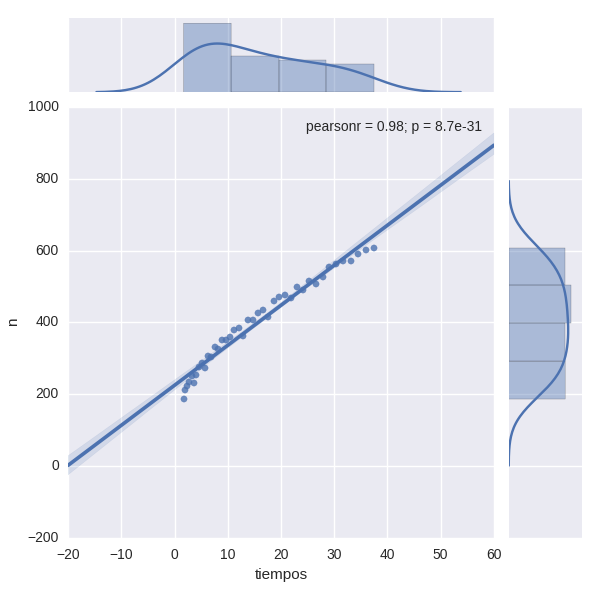
\includegraphics[width=8cm,height=8cm,keepaspectratio]{img/testk_n.png}}
\hspace*{-1cm}{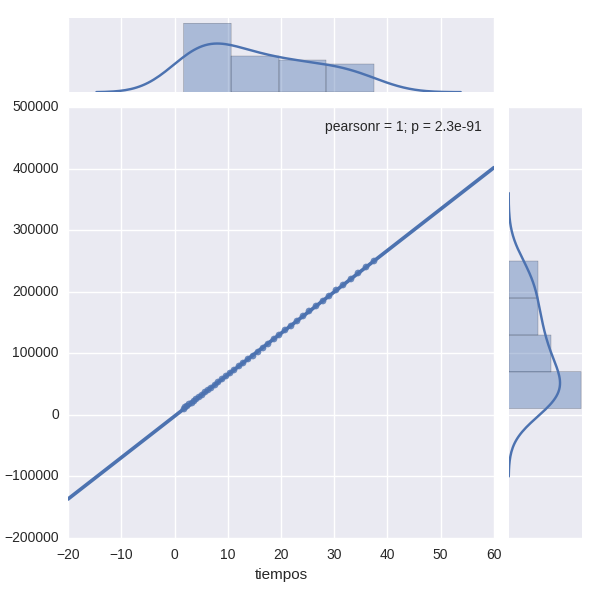
\includegraphics[width=8cm,height=8cm,keepaspectratio]{img/testk_n2.png}}

\hspace*{-1cm}{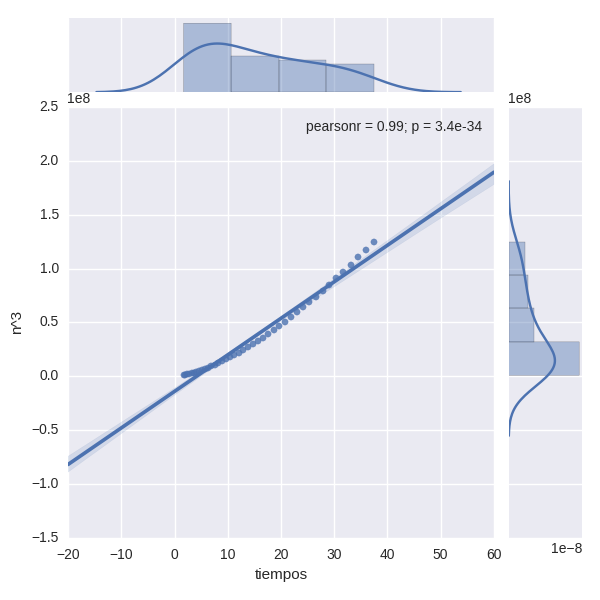
\includegraphics[width=8cm,height=8cm,keepaspectratio]{img/testk_n3.png}}
\hspace*{-1cm}{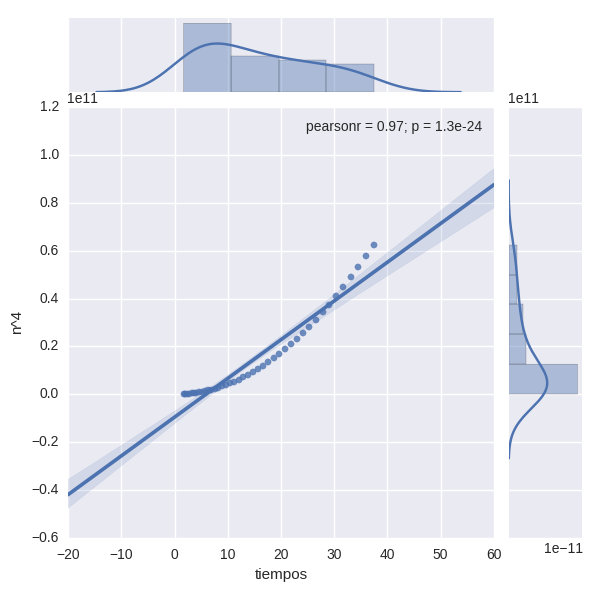
\includegraphics[width=8cm,height=8cm,keepaspectratio]{img/testk_n4.png}}

Nuevamente la correlación entre los tiempos obtenidos y $n^2$ es perfecta, indicando que el crecimiento de la función es cuadrático en $k$. Nuevamente la correlación con $n^3$ es casi perfecta (y con mayor margen de error), sugiriendo, al igual que $n$, la diferencia será más notoria con muestras mayores debido a las constantes que acompañan a las funciones de complejidad. 


\paragraph{Complejidad sobre $m'$}

Se fijarán $n$ y $k$ en 1000 y 20 y $m'$ se moverá entre 1000 y 4950 dando saltos de a 50. Nuevamente se realizarán 5 repeticiones y se tomará la mediana de los tiempos obtenidos. En cuanto al resultado esperado, se espera que el crecimiento sea lineal con respecto a $n$, por lo que en este caso los tiempos de corrida se correlacionarán con la función constante y con las funciones $n$, $n^2$ y $n^3$. A continuación presentamos los resultados:

\hspace*{-1cm}{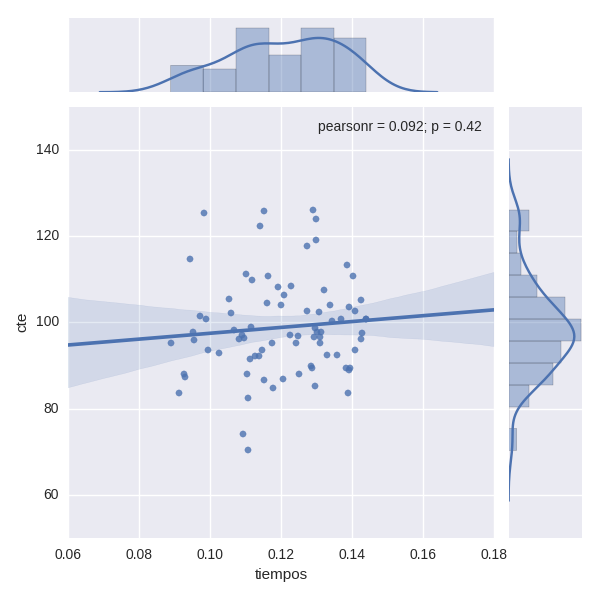
\includegraphics[width=8cm,height=8cm,keepaspectratio]{img/testm_cte.png}}
\hspace*{-1cm}{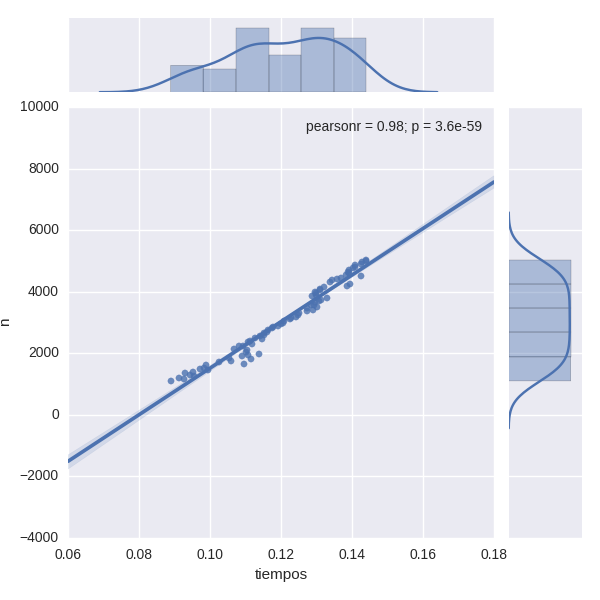
\includegraphics[width=8cm,height=8cm,keepaspectratio]{img/testm_n.png}}

\hspace*{-1cm}{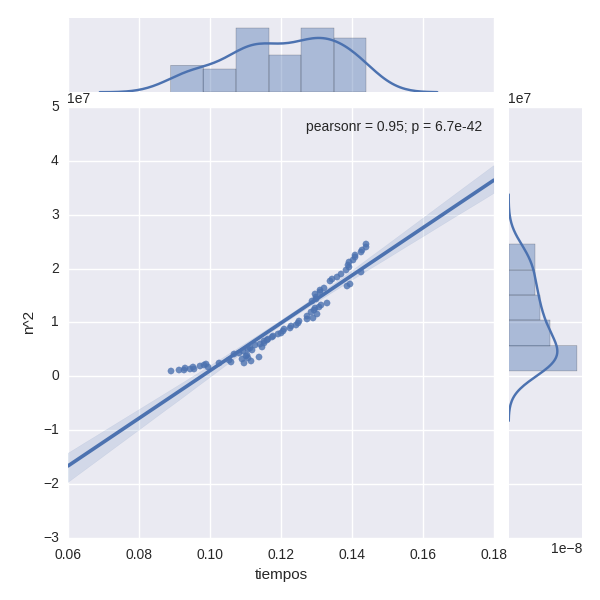
\includegraphics[width=8cm,height=8cm,keepaspectratio]{img/testm_n2.png}}
\hspace*{-1cm}{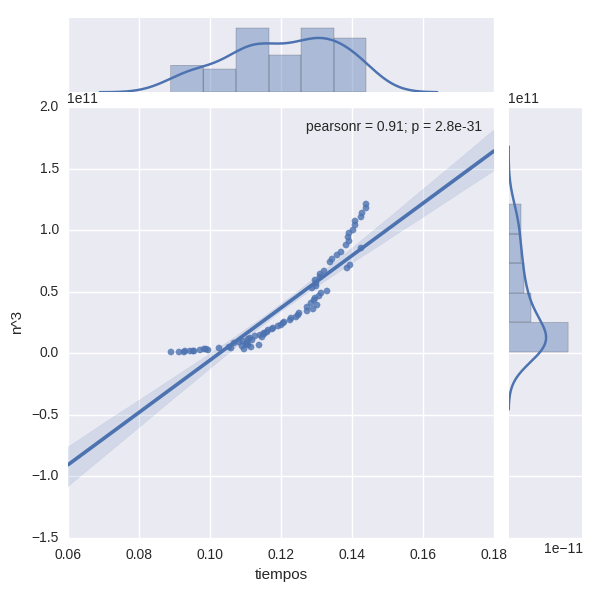
\includegraphics[width=8cm,height=8cm,keepaspectratio]{img/testm_n3.png}}

Si bien ninguna de las funciones expuestas se correlaciona perfectamente con los tiempos obtenidos (cosa que \textit{si} pasaba en los casos anteriores, la función lineal es la que mejor correlación, sugiriendo que afirmar que el crecimiento es lineal con respecto a $m$ es lo más cercano a la realidad. Notar que como $m \in $ O($n^2k^2$), podría usarse esta última cota de complejidad para toda la solución, lo cual sugeriría que el crecimiento en $m$ tendría que ser constante. Sin embargo, observar que la función constante esta muy poco correlacionada con los tiempos obtenidos, por lo que utilizar esta cota sería perder información sobre los tiempos reales del algoritmo. 


\subsubsection{Casos buenos y malos}

En nuestra implementación del algoritmo de Dijkstra agregamos un corte para que, una vez que un nodo que contenga la ciudad de destino sea desencolado, el algoritmo pare y devuelva la distancia hallada. Mediremos esta condición de corte con un gráfo de ?? nodos que consistirá en un único camino. Así, si $G=(V,X)$ es el éste grafo, $V=\{n: 1 \leq n \leq 5000\}$ y $X=\{ (i, i+1) : 0 \leq i \leq 5999 \}$. Fijaremos $k$ en 2, sin embargo ninguna ruta será premium. Así, $n$, $m$ y $k$ quedan fijados en 5000, 4999 y 2 respectivamente. Estableceremos al nodo 1 como origen e iremos moviendo el nodo de destino desde 1000 hasta 5000 aumentando de a 100. Mediremos los tiempos de corrida, corriendo cada caso 5 veces y tomando la mediana:

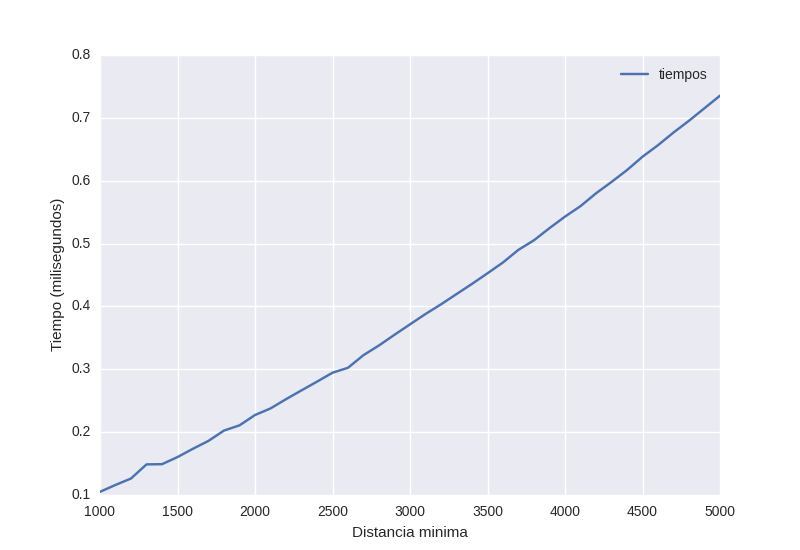
\includegraphics[width=15cm,height=15cm,keepaspectratio]{img/caso_dist.png}

La variación de tiempos es lineal porque en los casos de test el destino cambia (crece) de forma lineal. Lo importante en este caso no es el tipo de crecimiento sino que efectivamente se observan cambios en los tiempos de corrida del algoritmo. Esto quiere decir que, gracias a la condición de corte extra en el algoritmo de Dijkstra, el tiempo total que tarda en correr el algoritmo se reduce según el camino mínimo que se esté buscando. Dicho de otra forma, si el nodo de destino es encontrado rápidamente, solo estaremos obligados a pagar el costo de armar el digrafo, sumado a las iteraciones que haga Dijkstra. Si bien esto no cambia las complejidades teóricas, sí podemos afirmar que en la práctica pueden lograrse tiempos mejores que los analizados. 






\end{subsection}

